% ==========================================================================
%  PARTE II — MARCO DE ESTIMACIÓN (sensibilidad + calibración bayesiana)
%  Secciones integradas al documento maestro. Mismo estilo y comandos que el
%  documento físico (\code, \fn, \src, \nota).
% ==========================================================================

% =====================================================
\section{Análisis de sensibilidad de las fuentes de incertidumbre}\label{sec:sensibilidad}
% =====================================================

El simulador de las secciones anteriores es el \emph{modelo directo}: dado un
conjunto de parámetros (potencia, posición y altura de las lámparas; propiedades
ópticas del agua) predice el campo de irradiancia. En la práctica varias de esas
entradas son inciertas a la vez, y antes de calibrarlas conviene saber
\emph{cuáles importan}. El análisis de sensibilidad (SA) cuantifica cómo la
incertidumbre de la salida se reparte entre las incertidumbres de las entradas.

\subsection{Local frente a global; la trampa del OAT}

El enfoque ingenuo —variar un factor a la vez (\emph{one-at-a-time}, OAT) alrededor
de un punto nominal— es \emph{local}: sólo explora un punto del espacio y no detecta
interacciones. Para un modelo no lineal como un trazador de rayos se requiere SA
\emph{global}: explorar conjuntamente todo el rango plausible de todas las entradas.
La Tabla~\ref{tab:sataxonomia} resume las familias de métodos.

\begin{table}[h]
\centering
\caption{Familias de análisis de sensibilidad y su ámbito de uso.}
\label{tab:sataxonomia}
\small
\begin{tabular}{lll}
\toprule
Familia & Qué mide & Costo / cuándo \\
\midrule
Local (derivadas en un punto) & $\partial y/\partial x_i$ nominal & barato; sólo local \\
Screening (Morris) & importancia y no-linealidad relativas & muy barato; jerarquizar \\
Varianza (Sobol, FAST) & fracción de varianza e interacciones & caro; aportes exactos \\
Derivadas globales (DGSM) & derivadas promediadas en todo el dominio & medio; cota de Sobol \\
Metamodelos (PCE, GP) & sustituto barato del modelo caro & medio; habilita lo anterior \\
\bottomrule
\end{tabular}
\end{table}

\subsection{Descomposición de varianza (Sobol / ANOVA--HDMR)}\label{sec:sobol}

El marco de referencia del SA global descompone la función en efectos de orden
creciente (descomposición ANOVA o HDMR):

\begin{equation}
f(\mathbf{x}) = f_0 + \sum_i f_i(x_i) + \sum_{i<j} f_{ij}(x_i,x_j) + \cdots,
\label{eq:hdmr}
\end{equation}

con términos mutuamente ortogonales. Tomando varianzas, la varianza total $V(y)$ se
reparte en contribuciones independientes, de donde surgen los \emph{índices de
Sobol}~\cite{sobol2001,saltelli2008}:

\begin{equation}
S_i = \frac{V_{x_i}\!\bigl[\,\mathbb{E}_{\mathbf{x}_{\sim i}}(y\mid x_i)\,\bigr]}{V(y)},
\qquad
S_{Ti} = 1 - \frac{V_{\mathbf{x}_{\sim i}}\!\bigl[\,\mathbb{E}_{x_i}(y\mid \mathbf{x}_{\sim i})\,\bigr]}{V(y)} .
\label{eq:sobol}
\end{equation}

El índice de primer orden $S_i$ es la fracción de varianza explicada por $x_i$ por
sí solo (efecto principal); el índice total $S_{Ti}$ incluye todas sus
interacciones. Su diferencia $S_{Ti}-S_i$ mide cuánto interactúa $x_i$ con las
demás; si $\sum_i S_i\approx1$ el modelo es casi aditivo. Estimar estos índices por
muestreo de Saltelli cuesta $N(2k+2)$ evaluaciones, prohibitivo para un simulador
estocástico.

\subsection{Por qué se muestrean derivadas del modelo}\label{sec:derivadas}

La sensibilidad elemental de una salida frente a una entrada es su derivada parcial
$\partial y/\partial x_i$, pero en un modelo no lineal ese valor cambia según dónde
se evalúe. Los métodos \emph{basados en derivadas globales} (Morris y
DGSM~\cite{kucherenko2009}) resuelven esto muestreando muchas derivadas por
diferencias finitas repartidas por todo el dominio y resumiéndolas
estadísticamente: el promedio del valor absoluto mide importancia global; la
dispersión mide no-linealidad e interacción (si la derivada fuese constante, el
factor sería lineal-aditivo). Es una aproximación muestral al gradiente que, sin el
costo de Sobol, ordena correctamente los factores —y la media de derivadas al
cuadrado (DGSM) acota por arriba al índice total de Sobol~\cite{kucherenko2009}.

\subsection{Método de Morris (efectos elementales)}\label{sec:morris}

Con el modelo normalizado $y=f(\mathbf{x})$, $\mathbf{x}\in[0,1]^k$, el
\emph{efecto elemental} del factor $i$ en $\mathbf{x}$ es la diferencia finita a lo
largo de la coordenada $i$~\cite{morris1991}:

\begin{equation}
EE_i(\mathbf{x}) = \frac{f(\mathbf{x}+\Delta\,\mathbf{e}_i) - f(\mathbf{x})}{\Delta}.
\label{eq:ee}
\end{equation}

El diseño de \emph{trayectorias} de Morris construye $r$ caminos, cada uno de $k+1$
puntos en los que cada factor se perturba exactamente una vez; así cada trayectoria
produce los $k$ efectos elementales con sólo $k+1$ evaluaciones (costo total
$r(k+1)$). Los índices por factor son la media de valores absolutos y la desviación
estándar~\cite{campolongo2007}:

\begin{equation}
\mu_i^{*} = \frac{1}{r}\sum_{t=1}^{r}\bigl|EE_i^{(t)}\bigr|
\quad\text{(importancia)},
\qquad
\sigma_i = \operatorname{std}\bigl(EE_i^{(t)}\bigr)
\quad\text{(no-linealidad/interacción)}.
\label{eq:mustar}
\end{equation}

\src{Screening de Morris con \code{SALib} en \fn{run\_screening.py}
(\code{sensitivity/}). Diseño de $r{=}20$ trayectorias, $p{=}4$ niveles, $k{=}6$
factores; forward determinista (semilla fija) para que $EE_i$ refleje física y no
ruido de Monte Carlo. Métrica de salida: desajuste robusto sim--medición por banda.}

\subsection{Por qué Morris en este problema}

Con seis fuentes de incertidumbre (potencia, posición y altura de las lámparas, y
los bio-ópticos $c_{550}$, $\omega$, $\eta$) y un modelo directo caro y
\emph{estocástico}, Sobol habría exigido miles de corridas ruidosas. El screening de
Morris, con $\sim$140 corridas deterministas, bastó para \emph{jerarquizar} las
fuentes y decidir dónde invertir la calibración. El resultado
(Figura~\ref{fig:morris}) es inequívoco: la bio-óptica domina el desajuste
($\mu^{*}$ de $c_{550}$ y $\omega$ muy por encima del resto; potencia y altura
$\sim$8\,\% cada una; posición $\sim$4\,\%). Sobol quedaría como refinamiento
posterior si se quisieran los porcentajes exactos de varianza.

\begin{figure}[h]
\centering
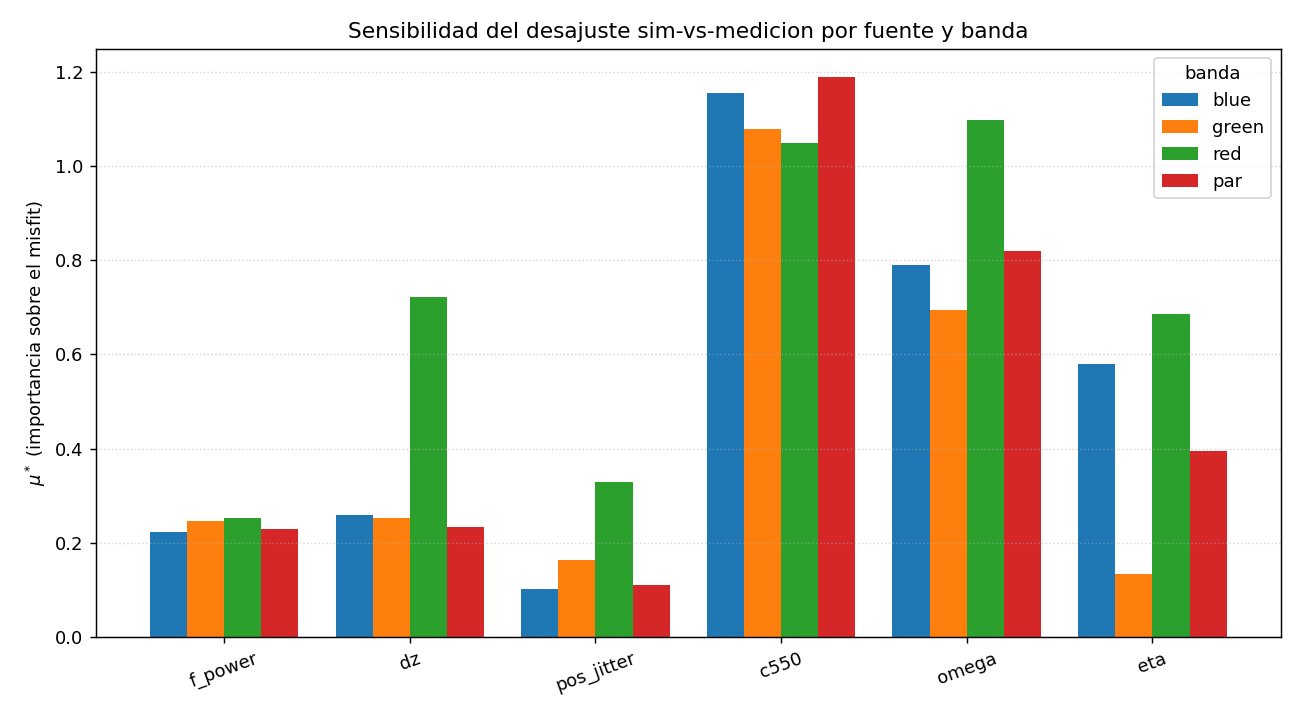
\includegraphics[width=0.82\linewidth]{../sensitivity/out/mu_star_misfit_por_banda.png}
\caption{Índices $\mu^{*}$ de Morris por fuente y banda espectral. La bio-óptica
($c_{550},\omega,\eta$) domina el desajuste sim--medición.}
\label{fig:morris}
\end{figure}

% =====================================================
\section{Calibración bayesiana de los parámetros bio-ópticos}\label{sec:bayes}
% =====================================================

Calibrar es un \emph{problema inverso}: de mediciones ruidosas y escasas se infieren
parámetros del agua que no se observan directamente. Estos problemas suelen ser mal
planteados —varias combinaciones de parámetros explican los datos casi igual—, lo
que motiva el marco bayesiano.

\subsection{Por qué el marco bayesiano encaja este problema}

Cuatro propiedades lógicas lo hacen el natural: (i) incorpora conocimiento previo
—priors físicos de $a$ y $b$ que regularizan la inversión mal planteada—; (ii)
cuantifica incertidumbre entregando distribuciones posteriores, no un único valor;
(iii) marginaliza coherentemente los parámetros de estorbo (\emph{nuisance}), como
la posición del sensor o la escala de potencia; y (iv) permite comparar modelos por
evidencia, con penalización de complejidad incluida.

\subsection{Fundamentos}

Todo descansa en el teorema de Bayes, posterior $\propto$ verosimilitud $\times$
prior:

\begin{equation}
p(\boldsymbol\theta\mid\mathbf{y}) = \frac{p(\mathbf{y}\mid\boldsymbol\theta)\,p(\boldsymbol\theta)}{p(\mathbf{y})},
\qquad
p(\mathbf{y}) = \int p(\mathbf{y}\mid\boldsymbol\theta)\,p(\boldsymbol\theta)\,\mathrm{d}\boldsymbol\theta,
\label{eq:bayes}
\end{equation}

donde $\boldsymbol\theta$ son los parámetros, $\mathbf{y}$ los datos, y
$p(\mathbf{y})$ la \emph{evidencia} (constante de normalización que sirve para
comparar modelos).

\subsection{Modelo de observación}

En $\log_{10}$, por sensor $i$ y banda $b$, con $g_b$ el trazador de rayos:

\begin{equation}
y_{i,b} = g_b(\mathbf{x}_i + \boldsymbol\delta_i;\ \boldsymbol\theta) + O + \varepsilon_{i,b},
\qquad \varepsilon_{i,b}\sim\mathcal{N}(0,\ s_i^2),
\label{eq:obsmodel}
\end{equation}

con $\boldsymbol\theta=(c_{550},\omega,\eta,d_z)$ los parámetros de interés, $O$ la
escala/potencia global (\emph{nuisance}), $\boldsymbol\delta_i$ el desplazamiento de
posición del sensor (variable latente por dato) y $\varepsilon$ la discrepancia más
ruido de medición. El término de discrepancia —calibrar reconociendo que el modelo
es imperfecto— es el marco de Kennedy--O'Hagan~\cite{kennedy2001}, aquí en versión
simplificada (discrepancia i.i.d.).

\subsection{Marginalización de la posición (suma gaussiana)}

La posición real del sensor se trata como variable aleatoria y se integra sobre su
prior. Discretizando la vecindad en candidatos $c$ con pesos $w_c\propto
p(\boldsymbol\delta_c)$, la verosimilitud del punto es una \emph{mezcla gaussiana}
—la misma estructura que la marginalización de hipótesis en detección y seguimiento:

\begin{equation}
p(\mathbf{y}_i\mid\boldsymbol\theta,O) = \sum_c w_c \prod_b
\mathcal{N}\!\bigl(y_{i,b};\ g_b(\mathbf{x}_i+\boldsymbol\delta_c;\boldsymbol\theta)+O,\ s_i^2\bigr).
\label{eq:mixlike}
\end{equation}

Las bandas azul y verde de un mismo punto comparten el mismo
$\boldsymbol\delta_c$ (posición física común); $O$ se perfila (verosimilitud
concentrada). La inclinación del sensor plano entra como varianza heteroscedástica
$s_i^2 = s_\text{disc}^2 + (k\tan\theta_i\,\sigma_\text{tilt})^2$ que crece con el
ángulo cenital de incidencia $\theta_i$.

\subsection{Cómputo: importancia, ESS y balance heuristic de Veach}\label{sec:mis}

Como el modelo directo es caro y determinista (semilla fija), no se usa MCMC sino
\emph{muestreo de importancia}: se proponen $\boldsymbol\theta^{(j)}$ de una
distribución $q$ y se ponderan por la verosimilitud; con prior uniforme, las
expectativas posteriores son promedios ponderados $W_j\propto
p(\mathbf{y}\mid\boldsymbol\theta^{(j)})$. La calidad se mide con el tamaño de
muestra efectivo~\cite{kong1994}:

\begin{equation}
\mathrm{ESS} = \frac{\bigl(\sum_j W_j\bigr)^2}{\sum_j W_j^2}.
\label{eq:ess}
\end{equation}

Cuando se combinan muestras de \emph{varias} propuestas (un barrido uniforme amplio
más un lote refinado gaussiano cerca del modo), el muestreo de importancia múltiple
(MIS) evita el sesgo y el doble conteo. La regla casi óptima es el \emph{balance
heuristic} de Veach \& Guibas~\cite{veach1995}: a cada muestra $\mathbf{x}$ se le
pondera por la probabilidad de que la \emph{mezcla de todas las propuestas} la
hubiera generado. Con $n_s$ muestras de la propuesta $q_s$, el peso de una muestra de
la estrategia $s$ es

\begin{equation}
w_s(\mathbf{x}) = \frac{n_s\,q_s(\mathbf{x})}{\sum_k n_k\,q_k(\mathbf{x})},
\label{eq:balance}
\end{equation}

de modo que cada muestra contribuye con $f(\mathbf{x})/m(\mathbf{x})$, donde
$m(\mathbf{x})=\tfrac1N\sum_k n_k q_k(\mathbf{x})$ es la densidad de mezcla. Ninguna
región se cuenta dos veces y cada propuesta aporta donde es buena: la uniforme
garantiza cobertura global y la gaussiana refina el pico. Veach demostró que este
esquema está a una constante aditiva pequeña del óptimo en varianza.

\subsection{Selección de modelo por evidencia}

Los hiperparámetros (dispersión de posición, de inclinación, parametrización
espectral) se eligen por evidencia $Z(\phi)=\int
p(\mathbf{y}\mid\boldsymbol\theta,\phi)\,p(\boldsymbol\theta)\,\mathrm{d}\boldsymbol\theta$,
aproximada por el promedio de las verosimilitudes sobre el barrido; el posterior
sobre $\phi$ es $\propto Z(\phi)$. Esto es Bayes empírico / comparación bayesiana de
modelos (el análogo del test de razón de verosimilitud generalizado en detección) e
incorpora el factor de Occam: un modelo más flexible sólo gana si su mejora de
ajuste supera la penalización por complejidad. Es lo que evita el sobreajuste al
decidir cuánta incertidumbre de posición admitir.

\src{Barrido Latin-hypercube~\cite{mckay1979} y calibración por importancia:
\fn{calibrate\_sweep.py}, \fn{calibrate\_infer.py} (Fase 2). Marginalización de
posición e inclinación con validación cruzada y MIS: \fn{attack\_sweep.py},
\fn{attack\_infer.py}, \fn{attack\_position\_curve.py} (Fase 3), en
\code{sensitivity/}.}

% =====================================================
\section{Aplicación y resultados: Punta Iglesia}\label{sec:resultados}
% =====================================================

\subsection{Datos}

Se emplearon 35 mediciones de un espectrorradiómetro OHSP-350 en una grilla nominal
$x\in\{5,10,15\}$, $y\in\{5,10,15,20\}$, $z\in\{8,10,12\}$~\si{\meter} dentro de una
jaula de $40\times40\times20$~\si{\meter} con seis luminarias TEMPEST 600~W. De cada
espectro se integraron bandas azul ($400$--$500$), verde ($500$--$600$) y roja
($600$--$700$~\si{\nano\meter}); la roja quedó en el piso del sensor y se descartó.
Trabajando en $\log_{10}$ quedaron 31 puntos válidos $\times$ 2 bandas.

\nota{Las mediciones se tomaron con los peces en la jaula. La biomasa dispersa,
absorbe y sombrea la luz de forma espacial y temporalmente variable —un efecto no
modelado por el simulador (agua limpia)— por lo que un ajuste moderado es esperable
y parte de él se confunde con la incertidumbre de posición.}

\subsection{Sensibilidad y aparición del piso de desajuste}

El screening de Morris (\S\ref{sec:morris}) mostró que la bio-óptica domina. La
calibración bayesiana de $(a,b)$ (Fase 2) entregó $a_{550}\approx0{,}095$,
$b_{550}\approx0{,}61$, $\omega\approx0{,}87$, pero reveló un \emph{piso}: el mejor
ajuste posible fue $R^2\approx0{,}42$ y ninguna combinación de $(a,b)$ superó
$0{,}45$. El parámetro óptico no era el factor limitante.

\subsection{El piso es la posición del sensor}

Marginalizando la posición del sensor como variable latente
(\eqref{eq:mixlike}), el ajuste validado cruzado (posición inferida sólo con la
banda azul, prediciendo la verde) subió de $0{,}45$ a $\approx0{,}88$. Que una banda
prediga la otra confirma que las correcciones de posición son físicas, no
sobreajuste. La Figura~\ref{fig:poscurve} muestra que un error de posición
\emph{modesto} basta: desde $R^2=0{,}41$ con posición nominal, $\sim$0,5~m combinados
dan $0{,}69$; $\sim$0,7~m dan $0{,}77$; $\sim$1~m dan $\approx0{,}86$. La ganancia se
satura más allá de $\sim$1~m —la evidencia premia esa holgura extra porque absorbe
discrepancia del modelo (peces incluidos), no porque el ajuste mejore. Las
correcciones de posición inferidas tienen mediana $1{,}3$~m (90\,\% por debajo de
2~m), magnitudes físicas para una sonda en línea. La inclinación resulta secundaria.

\begin{figure}[h]
\centering
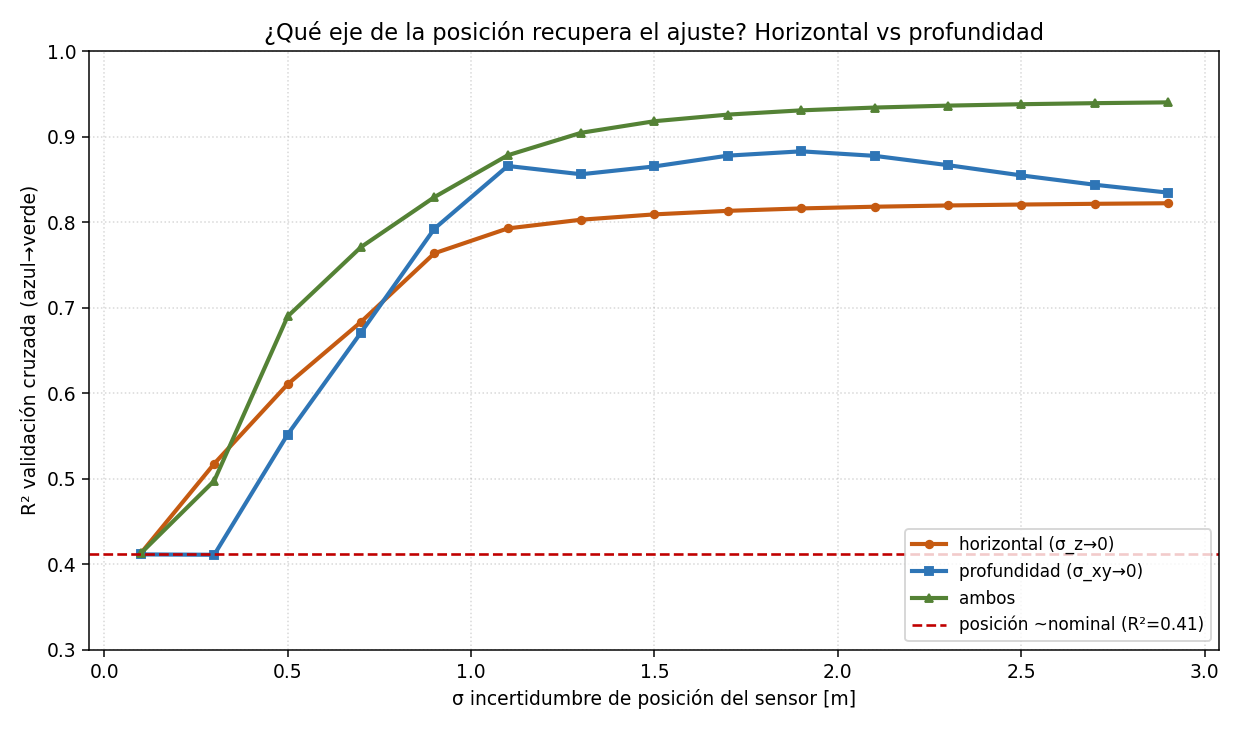
\includegraphics[width=0.80\linewidth]{../sensitivity/out/position_curve.png}
\caption{Ajuste validado cruzado frente a la incertidumbre de posición del sensor,
separando eje horizontal, profundidad y ambos. Un error combinado de $\sim$0,7--1~m
recupera la mayor parte del ajuste; no se requieren 2~m.}
\label{fig:poscurve}
\end{figure}

\subsection{Parámetros finales y estimación alternativa}

Al modelar la geometría de medición, el óptimo bio-óptico se desplaza respecto de la
Fase 2 (Tabla~\ref{tab:parametros}): ignorar la posición \emph{sesga} los
parámetros del agua. Se probó además una parametrización con pendientes espectrales
independientes para $a$ y $b$ ($a(\lambda)=a_{550}(\lambda/550)^{-\eta_a}$,
$b(\lambda)=b_{550}(\lambda/550)^{-\eta_b}$); no mejora el ajuste (0,90 frente a
0,88) y las dos pendientes salen casi iguales ($\eta_a\approx\eta_b\approx0{,}5$):
con sólo dos bandas los datos no pueden separar la forma espectral de la absorción de
la de la dispersión. En ambos casos la atenuación crece hacia el azul
(Figura~\ref{fig:espectral}), coherente con agua con partículas y CDOM.

\begin{table}[h]
\centering
\caption{Parámetros bio-ópticos estimados a 550~\si{\nano\meter} (mediana
posterior).}
\label{tab:parametros}
\small
\begin{tabular}{lccc}
\toprule
Parámetro & Fase 2 (posición ignorada) & Fase 3 (posición modelada) & Pendientes indep. \\
\midrule
$a_{550}$ [\si{\per\meter}] & 0,095 & 0,356 & 0,29 \\
$b_{550}$ [\si{\per\meter}] & 0,611 & 0,703 & 1,00 \\
$c_{550}=a{+}b$ [\si{\per\meter}] & 0,738 & 1,092 & 1,29 \\
$\omega=b/(a{+}b)$ & 0,874 & 0,646 & 0,77 \\
$\eta$ (o $\eta_a/\eta_b$) & 0,64 & 0,35 & 0,47 / 0,53 \\
$R^2$ validado (azul$\to$verde) & 0,42$^{*}$ & 0,88 & 0,90 \\
\bottomrule
\end{tabular}
\end{table}

\begin{figure}[h]
\centering
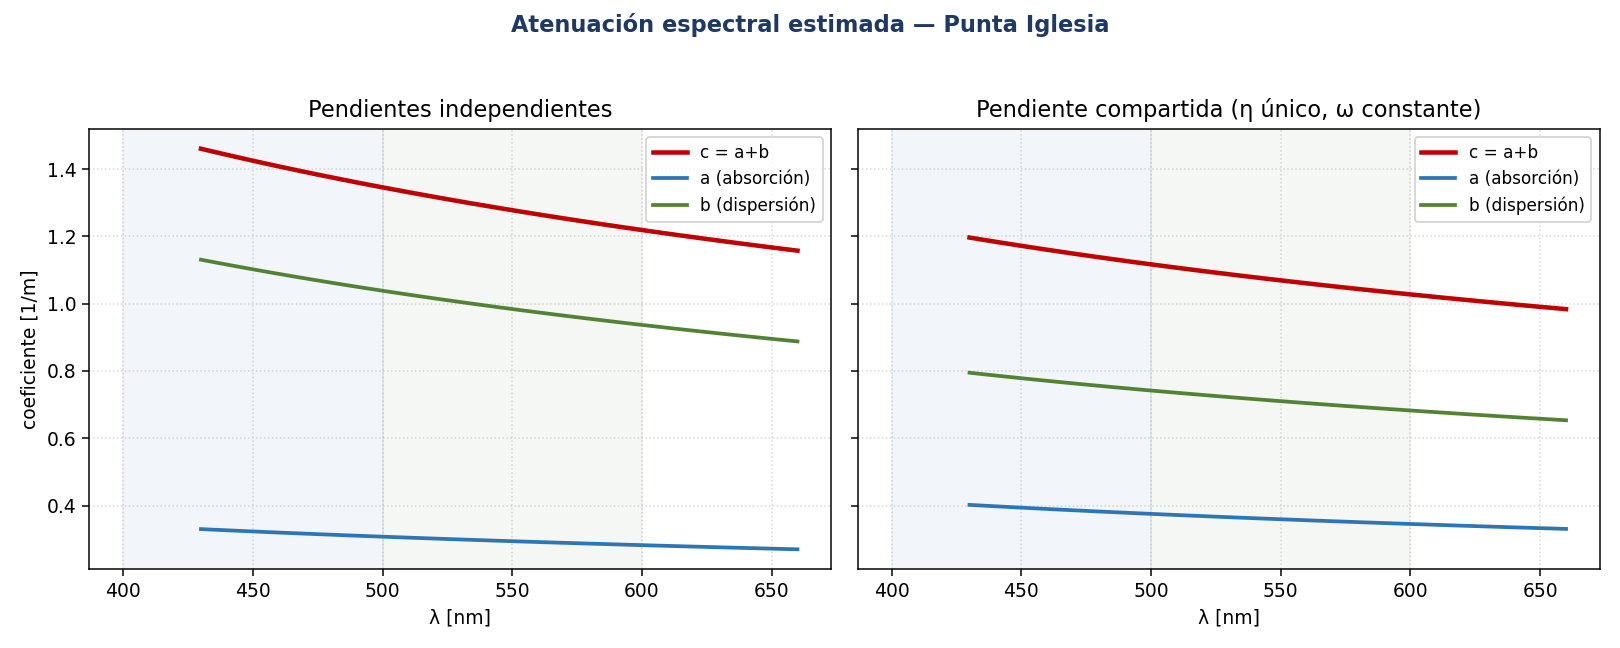
\includegraphics[width=0.92\linewidth]{../sensitivity/out/spectral_attenuation.png}
\caption{Atenuación espectral estimada $a(\lambda)$, $b(\lambda)$, $c=a+b$: modelo de
pendientes independientes (izq.) y de pendiente compartida (der.).}
\label{fig:espectral}
\end{figure}

\nota{Los parámetros de la Fase 3 son los preferidos, pero condicionados al modelo
de posición y con identificación limitada (el muestreo de importancia se satura,
$\mathrm{ESS}\to$ bajo). El valor $R^2\approx0{,}42$ marcado con $^{*}$ es el techo
de la Fase 2 sin modelar posición. El cuello de botella es metrológico: registrar
posición e inclinación del sensor, o medir $(a,b)$ in situ, rompería la confusión.}
